\documentclass{beamer}
\usepackage{tikz}
\usetikzlibrary{arrows.meta}
\usetheme{Rochester}

\title{TIPE 25/26 - Cycles et Boucles}
\author{GIL Dorian}
\subtitle{Méthode des tableaux : Optimisation pour des formules de la forme (?)}
\date{}

\begin{document}

\begin{frame}
\titlepage
\end{frame}

\begin{frame}{Sommaire}
\begin{enumerate}
    \item Présentation Méthode
    \item Exemple d'Application
    \item Implémentation en OCaml
    \item Objectifs futurs
\end{enumerate}
\end{frame}

\begin{frame}{Présentation}
    On souhaite prouver une formule dans la logique propositionelle :
    \begin{definition}[Méthode des tableaux]
        Méthode par laquelle on prouve une assertion $B$ ayant pour hypothèse $(A_n)$ en montrant
        que $\{A_1,\dots,A_n, \lnot B\}$ est insatisfaisable (Cela revient à montrer qu'une implication est vraie car sa négation ne peut être vraie).
    \end{definition}
    \pause
    \begin{itemize}
        \item On place $\lnot\phi$ et ses hypothèses dans la racine.
        \item On applique des règles $(R_x)$ à chaque formule en bout d'arbre qui sont developpables
        \item Si on trouve $a$ et $\lnot a$ dans l'arbre (un \textit{cycle}), alors $\phi$ est vrai
    \end{itemize}
    \pause
    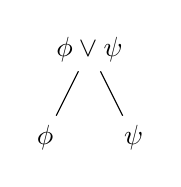
\begin{tikzpicture}[scale=0.75]
    \node {$\phi\lor\psi$}
        child {node {$\phi$}}
        child {node {$\psi$}};
    \end{tikzpicture}
    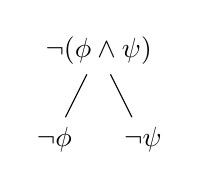
\begin{tikzpicture}[scale=0.75]
    \node {$\lnot(\phi\land\psi)$}
        child {node {$\lnot\phi$}}
        child {node {$\lnot\psi$}};
    \end{tikzpicture}
    \begin{tikzpicture}[scale=0.75]
    \node {$\lnot\lnot\phi$}
        child {node {$\phi$}};
    \end{tikzpicture}
    \begin{tikzpicture}[level distance=8mm]
    \node {$\phi\land\psi$}
        child {node {$\phi$} edge from parent }{
        child {node {$\psi$} edge from parent[draw=none]}};
    \end{tikzpicture}  
    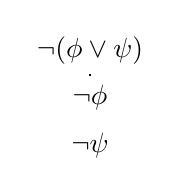
\begin{tikzpicture}[level distance=8mm,scale=0.75]
    \node {$\lnot(\phi\lor\psi)$}
        child {node {$\lnot\phi$} edge from parent }{
        child {node {$\lnot\psi$} edge from parent[draw=none]}};
    \end{tikzpicture}
    Les règles
\end{frame}


\begin{frame}{Exemple}
    \textbf{Formule:} $a \Rightarrow (b \Rightarrow a)$

    \begin{center}
        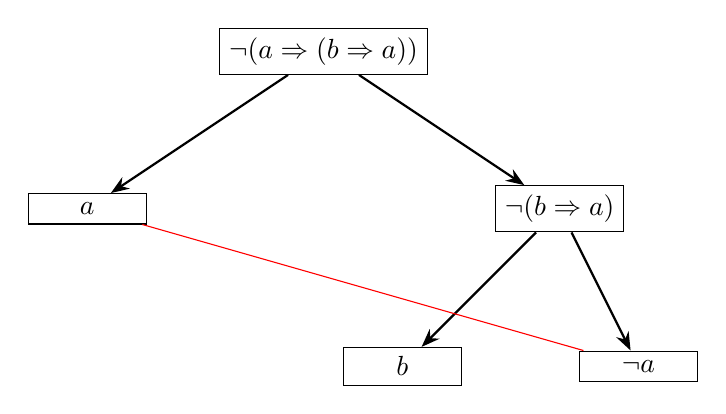
\begin{tikzpicture}[
            every node/.style={draw, minimum width=1.5cm, align=center},
            every arrow/.style={thick,->,>=Stealth}
        ]
        \node (root) at (0,0) {$\lnot(a \Rightarrow (b \Rightarrow a))$};
        \pause
        \node (a) at (-3,-2) {$a$};
        \node (not_b_a) at (3,-2) {$\lnot(b \Rightarrow a)$};
        \draw[every arrow] (root) -- (a);
        \draw[every arrow] (root) -- (not_b_a);
        \pause
        \node (b) at (1,-4) {$b$};
        \node (not_a) at (4,-4) {$\lnot a$};
        \draw[every arrow] (not_b_a) -- (not_a);
        \draw[every arrow] (not_b_a) -- (b);
        \pause
        \draw[red] (a) -- (not_a);
        \end{tikzpicture}

        On trouve un \textcolor{red}{cycle} $a\leftrightarrow \lnot a$. Cette négation de la formule est insatisfaisable,
        donc la formule a été prouvé.

    \end{center}
\end{frame}

\begin{frame}{Implémentation}
    Le code
\end{frame}

\begin{frame}{Ce qui est à faire}
    Mon but sur le long terme
    \begin{itemize}[<+->]
        \item Implémenter les tableaux en logique propositionelle
        \item Trouver et prouver des optimisations pour les formules (?)
        \item Implémenter et commenter les résultats de l'optimisation
        \item Faire de même cette méthode en logique du première ordre OU continuer à trouver des optimisations dans la logique propositionelle
    \end{itemize}
    Sur le court terme :
    \begin{itemize}[<+->]
        \item One
        \item Two
    \end{itemize}
\end{frame}
\end{document}